\documentclass[11pt,a4paper]{article}
\usepackage{graphicx}
\usepackage{sidecap}
\usepackage{mathtools}
%Om grotere integralen te krijgen
\usepackage{relsize}
\usepackage[dutch]{babel}

%Andere breedte en lengthe van een document
\setlength{\textwidth}{6in} 
\addtolength{\hoffset}{-0.5in}
\setlength{\topmargin}{-0.2in}
\setlength{\textheight}{9in}

%Packages voor de figuren:
\usepackage{wrapfig}
\usepackage{caption}
\usepackage{subcaption}
%Kan er voor zorgen dat een figuur op de exacte plaats staat:
\usepackage{float}

%Package voor algoritmen:
\usepackage{algpseudocode}
\usepackage{algorithm}
\begin{document}
\begin{titlepage}

\title{\Huge Toepassingen van meetkunde in de informatica}

\author{Robin Goots\\
		Ward Schodts\\
		}

\date{2013 - 2014}
\maketitle
\thispagestyle{empty}


\begin{center}
\Large Professor Dirk Roose
\vfill
\end{center}
\end{titlepage}
\section{De onderzoeksvraag}
Hoe kunnen we de snijpunten van N cirkels vinden? 
\begin{enumerate}
\item Wat zijn de verschillende algoritmen?
\item Wat is de rekencomplexiteit van deze algoritmen?
\item In welke omstandigheden presteert het ene algoritme beter als het andere?
\end{enumerate}
\section{Hoogniveau beschrijving van de algoritmen}
\subsection{Algoritme 1}
Het eerste algortime is een brute-force algoritme. In essentie neemt het \'e\'en van de N cirkels en gaat het dan deze cirkel vergelijken met elke andere cirkel. Om zo te controleren of de cirkels overlappen en dusdanig \'e\'en of twee punten gemeenschappelijk hebben.
\\
\\
De complexiteit van het algoritme kan theoretisch gevonden worden op de volgende manier: er zijn $N$ cirkels, de eerste wordt gecontroleerd met $N-1$ anderen, de volgende met $N-2$ anderen, enzovoort. Dit geeft dus het volgende aantal controles:
$$(N-1) + (N-2) + (N-3) + (N - 4) \cdots $$
Dit is de som van de eerste $N-1$ getallen:
$$ = \frac{N\cdot (N-1)}{2} $$
Dit komt dus overeen met een rekencomplexiteit $O(N^2)$
\begin{algorithm}
\caption{eenvoudig algoritme met rekencomplexiteit $O(N^2)$}
\begin{algorithmic}
\State Lijst L met alle cirkels
\State Lijst ouput (met alle berekende snijpunten tussen de cirkels) = $\emptyset$
\While {Niet leeg L}
	\State Cirkel = L.NeemEnVerwijder()
	\For {c in L}
	\State snijptn = Cirkel.BerekenSnijpunten(c)
	\State output.VoegToe(snijptn)
	\EndFor
\EndWhile

\Return output
\end{algorithmic}
\end{algorithm}
\\
De functie \verb|NeemEnVerwijder()| geeft het eerste element van de lijst terug en verwijdert het daarna.\\
De functie \verb|BerekenSnijpunten(Cirkel c)| neemt als argument een cirkel aan en berekent de snijpunten met deze cirkel op de een andere cirkel waar deze methode werd uitgevoerd.

\subsubsection{Complexiteit}
De complexiteit van het algoritme kan theoretisch gevonden worden op de volgende manier: er zijn $N$ cirkels, de eerste wordt gecontroleerd (op snijpunten) met $N-1$ anderen, de volgende met $N-2$ anderen, enzovoort. Dit geeft dus het volgende aantal controles:
$$(N-1) + (N-2) + (N-3) + (N - 4) \cdots $$
Dit is de som van de eerste $N-1$ getallen:
$$ = \frac{N\cdot (N-1)}{2} $$
Dit komt dus overeen met een rekencomplexiteit $O(N^2)$
\subsubsection{Randvoorwaarden}
Voor dit algoritme leggen we als voorwaarde op dat er geen twee cirkels exact op elkaar mogen liggen. Dan krijgen oneindig veel snijpunten. 

\subsection{Algoritme 2}
\subsubsection{Algemeen}
Voor het volgende algoritme stellen we elke cirkel voor als een lijnstuk met als links eindpunt het meest linkse punt van de cirkel en als rechts eindpunt het meest rechtse eindpunt van de cirkel. Deze twee punten worden bij in het object cirkel opgelsagen. Al deze $2\cdot N$ punten worden gesorteerd op laagste x-coördinaat, daarna op laagste y-coördinaat, en uiteindelijk op het feit of dat het een links uiterste rechts uiterste is van de cirkel.
\\
\\
Dit algoritme gebruikt een doorlooplijn. De gesorteerde lijst wordt afgegaan, telkens wanneer we een links punt van een cirkel tegenkomen voegen we dit toe aan een tweede lijst. Indien we een rechts punt tegenkomen wordt dit punt uit deze tweede lijst verwijderd. Vanaf de moment dat er een cirkel wordt toegevoegd aan de tweede lijst dan wordt deze cirkel met alle andere cirkels in de lijst vergeleken om te controleren of er geen snijpunten zijn.
\subsubsection{Hoogniveau beschrijving}
\begin{algorithm}
\caption{doorlooplijnalgoritme met rekencomplexiteit $O(N^2)$}
\begin{algorithmic}
\State Lijst L: een gesorteerde lijst met $2N$ punten.
\State Lijst C: met alle cirkels op een bepaald moment van een eventpoint, ongesorteerd.


\For {elk punt p in L}
	\If {p is het linkse eindpunt van een lijnstuk c}
	
		\State snijptn = Cirkel.BerekenSnijpunten(c)
		\State output.VoegToe(snijptn)	
		\State VoegToe(C,c)

	\Else
		\State Verwijder(C,c)
	\EndIf
\EndFor

\Return output
\end{algorithmic}
\end{algorithm}
Het punt waar de doorlooplijn zich bevindt wordt een evenpoint genoemd.\\
De methode \verb|BerekenSnijpunten(Cirkel c)| is net hetzelfde als in algortime 1.
\subsubsection{Complexiteit}
De 
\subsubsection{Randvoorwaarden}
\subsection{Algoritme 3}
\subsubsection{Algemeen}
Voor dit algoritme hebben we een benadering van $O((N+R)Log(N)$
\subsubsection{Hoogniveau beschrijving}
\begin{algorithm}
\caption{complex doorlooplijnalgoritme met rekencomplexiteit $O((N+S)Log(N))$}
\begin{algorithmic}
\State Lijst L: een gesorteerde lijst met $2N$ punten.
\State Lijst S: met alle segmenten op een bepaald moment van een eventpoint, ongesorteerd.
\For {elk punt p in de gesorteerde lijst}
	\If {p is het linkse eindpunt van een cirkel c}
	
		\State snijptn = Cirkel.BerekenSnijpunten(c)
		\State output.VoegToe(snijptn)
	
	\State VoegToe(C,c)
	\EndIf
	\If {p is het rechtse eindpunt van een cirkel c}
	\State Verwijder(C,c)
	\EndIf
\EndFor

\Return output
\end{algorithmic}
\end{algorithm}

\section{Correctheid van de algoritmen verifi\"eren}

Om de correctheid van de algoritmen te verifi\"eren hebben we verschillende stappen ondernomen. Deze stappen moeten in chronologische volgorde worden uitgevoerd omdat we assumpties uit voorgaande stappen gebruiken om te huidige stap te verifi\"eren.

\subsection{Enkele manuele testen}

\subsubsection*{bepalen dat cirkels snijden}
Onze eerste zorg was er zeker van zijn dat onze methode voor het bepalen dat cirkels snijden correct werkt. Met behulp van internet hebben we formules afgeleid om te bepalen of cirkels snijden. Na dat we deze formules afgeleid hebben, hebben we deze omgezet in Python code.

\subsubsection*{Bepalen van snijpunten van twee cirkels}
Na dat we er zeker van zijn dat onze cirkels snijden of niet moeten we bepalen waar deze snijden. Wederom hebben we met behulp van internet formules afgeleid om de snijpunten van circels te bepalen. Deze keer hebben we ook tussenstappen bepaald om te berekenen dat er \'e\'en of twee snijpunten zijn. Deze formules hebben we ook omgezet in Python code.

\subsubsection*{Algoritme 1}

Aangezien in algoritme \'e\'en alle cirkels met alle andere cirkels vergeleken worden gaan we zeker geen snijpunten missen. Verder hebben we ook al bewezen dat het bepalen dat cirkels snijden en de bepaling van eventuele snijpunten correct zijn. Uit deze twee stellingen kunnen we concluderen dat algoritme \'e\'en correct is.
Om eventuele bugs in de code uit te sluiten hebben we een klein aantal cirkels handmatig berekend. Dit resultaat hebben we vergeleken met het resultaat dat onze code ons geeft.

\subsubsection*{Algoritme 2}


Het is niet zo eenvoudig om te bewijzen dat algoritme twee correct is. De code voor het bepalen dat twee cirkels snijden en het berekenen van de snijpunten hergebruiken we. Op deze manier zijn we zeker dat hier geen fout inzit.
Aangezien algoritme \'e\'en correct is moeten we met algoritme twee dezelfde uitkomst krijgen als we dezelfde invoer gebruiken. Dit maakt het verifi\"eren van de correctheid al een stuk eenvoudiger.

Als eerst hebben we de uitkomst van algoritme \'e\'en en twee naast elkaar geplakt in een rekenblad. Nadat we beide uitkomstensets gesorteerd hebben, hebben we een paar steekproeven genomen om te controleren of deze dezelfde zijn. Dit bleek zo te zijn. In dit zelfde rekenblad hebben we ook de som genomen van de x-waarden en de y-waarden. Deze twee sommen blijken ook overeen te komen. Uit deze twee proeven kunnen we concluderen dat de resultaten voor beide algoritmen overeen komen.

Na deze numerieke test hebben we ook nog een visuele test uitgevoerd. De resultaten die de algoritmes terug geven zijn eenvoudig om te zetten naar een Scalable Vector Graphics bestand. In dit bestand hebben we eerst alle snijpunten die algoritme \'e\'en opleverd geschreven in \'e\'en bepaalde kleur. Daarna alle snijpunten die algoritme twee opleverd in een andere kleur. Aangezien enkel het laatst geschreven punt zichtbaar is, kunnen we makkelijk visueel controleren dat algoritme twee alle snijpunten vind door te controleren dat het geplotte svg bestand maar \'e\'en kleur weergeeft.

\begin{figure}[H]
\centering
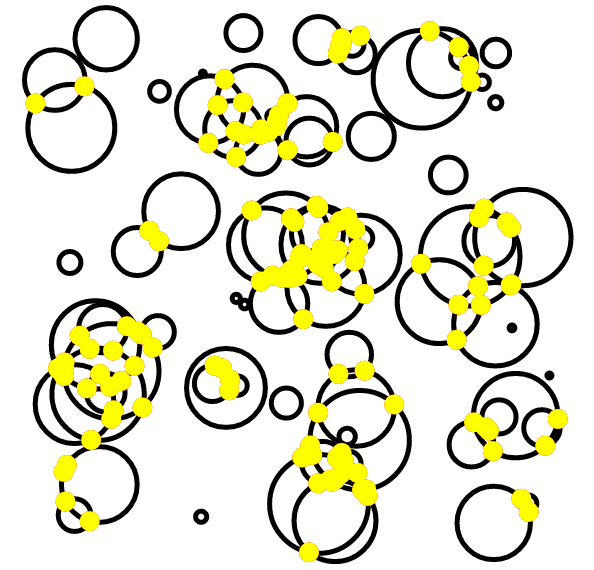
\includegraphics[width=0.5\textwidth]{vb_svg.png}
\caption*{Voorbeeld van een svg die gegenereerd word}
\end{figure}

De numerieke en visuele test hebben we meermaals uitgevoerd met verschillende parameters voor de random gegenereerde cirkels om er zeker van te zijn dat onze testen niet toevallig slagen.

\subsubsection*{Algoritme 3}

De correctheid van algoritme drie gaan we op dezelde manier bepalen als algoritme twee. De code voor het bepalen dat cirkels snijden en het berekenen van snijpunten hergebruiken we wederom.

Als we de uitkomsten van algoritme \'e\'en en drie in een rekenblad plakken valt ons voor grote aantallen cirkels onmiddelijk op dat algoritme \'e\'en en drie niet hetzelfde aantal snijpunten vinden. Hieruit vermoeden we al dat algoritme drie niet correct werkt.

Ook de visuele test bevestigd ons vermoeden uit de numerieke test. De visuele test brengt wel een interessant gegeven aan het licht. Alle snijpunten die niet gevonden worden blijken in gebieden bij elkaar te liggen. (Zoals blijkt op onderstaande figuur.) Dit geeft ons het vermoeden dat er een fout zit in onze methode die de boom doorloopt opzoek naar snijdingen met het opgegeven segment.

\begin{figure}[H]
\centering
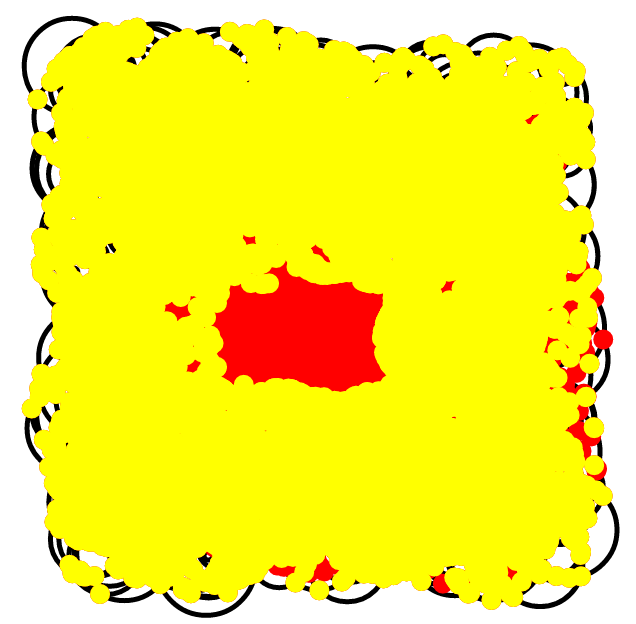
\includegraphics[width=0.5\textwidth]{gat_midden.png}
\caption*{Svg die een gebied bevat van snijpunten die niet gevonden worden}
\end{figure}

Bij nader onderzoek van de code komen we tot de vaststelling dat hoogstwaarschijnlijk onderstaand stuk code verantwoordelijk is voor de foutieve werking. Indien we \\ \verb|nodeQueue.put(current.left)| uitcommenten in de eerste if en commenten in de tweede if blijkt dat algoritme drie correct werkt. Op deze manier hebben we algoritme drie terug gereduceerd tot $O(n^{2})$ in het slechtste geval aangezien we elke cirkel terug gaan vergelijken met alle mogelijke cirkels die kunnen snijden.

\begin{verbatim}
if current.left is not None:
    #nodeQueue.put(current.left)
    if current.left.maxhi >= interval.lo.yco:
        nodeQueue.put(current.left)
                
\end{verbatim}

Uit dit onderzoek komen we tot de conclusie dat er takken van de zoekboom worden afgesneden die we wel moeten bezoeken. Dit wordt mogelijks veroorzaakt door een verkeerde maxhi waardoor er een cutoff ontstaat in de intervaltree waar er geen zou mogen zijn.

\section{Onderzoeksmethode}


\end{document}